\section{Introduction}
In this work we attempt the reproduction of the results presented in the paper "Dynamic Routing Transformer Network for Multimodal Sarcasm Detection" \cite{tian-etal-2023-dynamic}, which proposes DynRT, a new architecture to tackle the sarcasm detection task. The authors of the paper leverage multimodal NLP to join information obtained from pictures and their corresponding captions. 

\section{Scope of reproducibility}
\label{sec:claims}

The authors of the paper claim that their model outperforms the state-of-the-art models in the sarcasm detection task. They also claim that their model is able to leverage multimodal information to improve the overall performance in terms of both accuracy ad F1 score.
Ciao.The novel DynRT architecture is used to capture incongruity between the picture and the caption, which is a key aspect of sarcasm, and is tested on a multimodal sarcasm detection dataset to compare the results with other state-of-the-art models.
 


%\jdcomment{To organizers: I asked my students to connect the main claims and the experiments that supported them. For example, in this list above they could have ``Claim 1, which is supported by Experiment 1 in Figure 1.'' The benefit was that this caused the students to think about what their experiments were showing (as opposed to blindly rerunning each experiment and not considering how it fit into the overall story), but honestly it seemed hard for the students to understand what I was asking for.}

\section{Methodology}
To reproduce the results stated in the original paper we mainly used the code made available by the authors in their public repository (https://github.com/TIAN-viola/DynRT). The instructions provided were partially incomplete, and the code needed some small adjustments. We used a Colab notebook to run the experiments, which allowed us to leverage the NVIDIA V100 GPU.

\subsection{Model description}
The DynRT model is composed of three main parts: two encoders and a dynamic routing transformer. The two encoders are used to encode the input text and the image features, and are respectively RoBERTa \cite{RoBERTa} for the text and ViT \cite{ViT} for the images. \\
The dynamic routing transformer is used to capture the incongruity between the two modalities. It is composed of a stack of $N$ layers, each of which is composed of a multi-head co-attention routing module, a multi-head self-attention module and a feed-forward network; each module is followed by a residual connection and a normalization layer. The transformer leverages hierarchical co-attention to module the incongruity between texts and images. The output of the encoders is fed to the dynamic routing transformer, which outputs a vector of \textit{routed features} that are used for the classification together with the \textit{image features}. The output of the classification is a vector containing the probabilities of the input being sarcastic or not. 

\subsection{Datasets}
The dataset used to evaluate the architecture is the Multimodal Sarcasm Detection (MSD) dataset, whose composition and split information are shown in table \ref{tab:MSD}.
\begin{table}
    \caption{MSD dataset composition and split information}
    \label{tab:MSD}
    \centering
    \begin{tabular}{|c c c c|}
        \hline
         & \textbf{Train} & \textbf{Development} & \textbf{Test} \\
        \hline
        Sarcastic & 8,642 & 959 & 959 \\
        Non-sarcastic & 11,174 & 1,451 & 1,450 \\
        Total & 19,816 & 2,410 & 2,409 \\
        \hline
    \end{tabular}
\end{table}
The dataset is not perfectly balanced, but it reflects the real-world distribution of sarcastic and non-sarcastic sentences. The dataset is composed of sentences and their corresponding images. The preprocessing operations performed on the dataset before feeding it to the model are the following:
\begin{itemize}
    \item Discard tweets with regular worlds, such as \textit{sarcasm, sarcastic, irony, jokes, humor, reposting, ironic, exgag}, and URLs
    \item replace mentions with the token \textit{<USER>}
\end{itemize}
The dataset can be downloaded from https://github.com/headacheboy/data-of-multimodal-sarcasm-detection.


\subsection{Hyperparameters}
The configuration used to run the experiments is pretty similar to the one used by the authors (i.e. the hyperparameters that could have influenced the performance of the model, such as the learning rate, the batch size, etc., were left unchanged) in order to perform a fair comparison of the results. The only difference in our runs was in the parallelization of the training process, which was not configured by default. Initially we tried without it, but the training process was excessively long. Therefore, we increased the number of workers to 10. This has been made possible by the computational power and capacity provided by the GPU that we used. In this way we could run the whole training process (15 epochs) in less than 4 hours. 

\subsection{Experimental setup and code}
Since we used a Colab notebook to run the experiments, we created a copy of our repository in a Google Drive folder, and we mounted the drive in the notebook. Then we tried installing the requirements in the way described in the readme.md of the original repository (https://github.com/TIAN-viola/DynRT) but we encountered some problems due to incompatible versions of some libraries. Therefore, we manually changed the installation process by updating the problematic libraries to their latest version. \\
We then proceeded to the preprocessing phase as shown by the authors, which consisted in performing the cleaning operations on the dataset and in converting the images to tensor. This last operation was performed locally, since we encountered some issues when trying to run it on the Colab notebook. We then uploaded the preprocessed dataset to the notebook and we started the training process. Here, we encountered other issues. Firstly, we had no feedback about how the training process was proceeding, therefore we decided to increase the verbosity by adding a code line that printed the advancement of the number of batches processed (with the default batch size of 32 we had to elaborate 611 batches for each epoch). Secondly, we got an exception due to the loading of some .npy files containing the tensors (previosly created starting from the images in the preprocessing phase). \\
Specificaly, some files couldn't be serialized in the way the algorithm was originally written. To solve this, we added an exception handling code block to manage these files. Finally, since Colab's stability is not complety reliable, we added a simple script in our notebook that leverages the checkpoint system implemented by the original authors: it checks whether a checkpoint file already exists or not, and if it does it loads the model from it (in case of multiple checkpoints models, it load the last one). \\
After these changes, we were able to run the training process without any other issues.


\subsection{Computational requirements}
As already mentioned, we used the NVIDIA V100 GPU provided by Colab Pro to run the experiments. The whole training and evaluation process took about 4 hours to complete, and we experienced a GPU memory consumption of about 4 GB. It is interesting to note how with no parallelization a single training epoch took about 3 hours to complete, which would have led to an excessively long training process of 45 hours for 15 epochs. This would have been an issue since Colab only allows for 12 hours of continuous execution.

\section{Results}
\label{sec:results}

\subsection{Results reproducing original paper}
The results obtained are in line with the ones provided in the paper. The authors report accuracy and F1 metrics obtained by averaging the performance of five different runs, showing how the newly introducted architecture outperforms other state-of-the-art models. The results that we obtained, shown in table \ref{tab:results} confirm those claims for accuracy results, but the F1 score obtained by us is slightly lower. 

\begin{table}
    \caption{Results obtained by the original authors and by us}
    \label{tab:results}
    \centering
    \begin{tabular}{| c|c c|}
        \hline
         & \textbf{Original} & \textbf{Reproduced} \\
        \hline
         \textbf{Accuracy} & 93.49 & 93.59 \\
        \hline
        \textbf{F1} & 93.21 & 91.93 \\
        \hline
    \end{tabular}
\end{table}

\section{Discussion}

Our experiment results match the ones reported in the paper, with a slight difference in the F1 score. This could be due to the fact that the authors averaged the results of five different runs, while we only performed one run. This could have led to a slightly different initialization of the model's weights, which could have influenced the final results. Anyway, the difference is not so significant, also because the F1 score obtained by us is still higher than the ones obtained by the other state-of-the-art models. \\ 
One interesting thing to note was how the performance of the model increased during the training process. As we can see from figure \ref{fig:accuracy} and \ref{fig:f1}, the accuracy and F1 score of the model were growing significantly slowlier during the first epochs, and then had a peak around the $11^{th}$ epoch. Our interpretation of this phenomenon is that the low learning rate used (1e-6) caused the model to get stuck in a local minimum, and then when it was able to get out of it, it started to learn faster, as shown by figure \ref{fig:loss}.

\begin{figure}[h]
    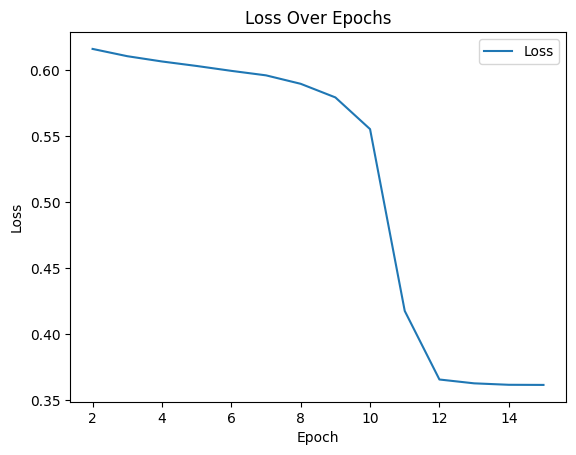
\includegraphics[width=8cm]{Loss.png}
    \label{fig:loss}
\end{figure}

\begin{figure}[h]
    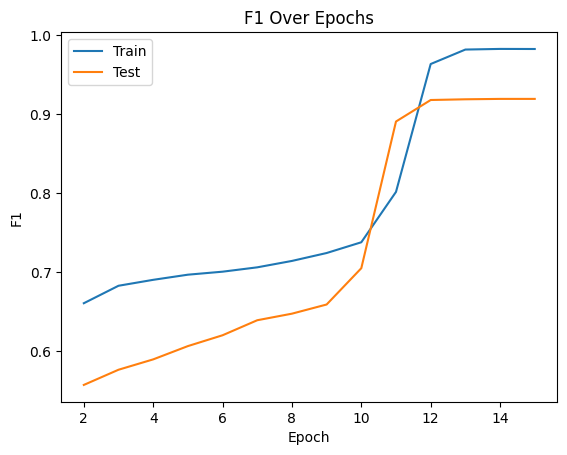
\includegraphics[width=8cm]{F1.png}
    \label{fig:f1}
\end{figure}

\begin{figure}[h]
    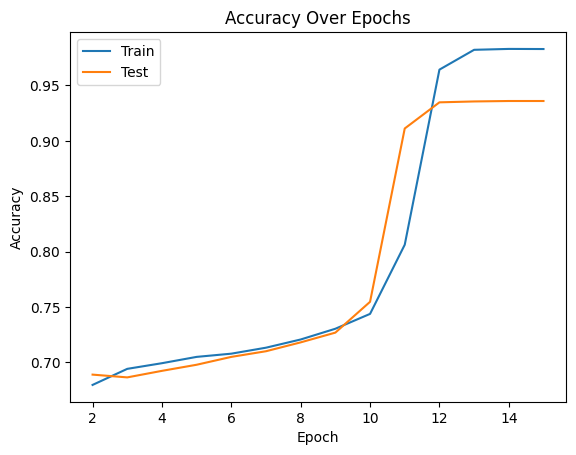
\includegraphics[width=8cm]{Accuracy.png}
    \label{fig:accuracy}
\end{figure}


\subsection{What was difficult}

The setup of the environment was not straightforward, since the instructions provided by the authors were outdated. We had to manually change the installation process of the requirements, and we had to add some code lines to the training process to make it work. This has been even more challenging because of the lack of comments in the code. \\
We also had to perform the preprocessing phase locally, since we encountered some issues when trying to run it on the Colab notebook. Also, it would have been interesting to compare the results in terms of precision and recall as well. Unfortunately this hasn't been possible since the authors didn't provide those metrics in their paper. 

\subsection{What was easy}
After having solved the issues concerning the setup of the environment, the training process was pretty straightforward. We only had to run the notebook and wait for the process to reach an end. Moreover, we managed to replicate the results stated in the paper directly using the configuration provided by the original authors. 


\subsection{Communication with original authors}
Since we managed to reproduce the results stated in the paper, we didn't have to contact the original authors.
